\documentclass[conference]{IEEEtran}
\IEEEoverridecommandlockouts
% The preceding line is only needed to identify funding in the first footnote. If that is unneeded, please comment it out.
\usepackage{cite}
\usepackage{amsmath,amssymb,amsfonts}
\usepackage{algorithmic}
\usepackage{graphicx}
\usepackage{textcomp}
\usepackage{xcolor}
\usepackage{hhline}
\usepackage{makecell}
\usepackage{multirow}
\def\BibTeX{{\rm B\kern-.05em{\sc i\kern-.025em b}\kern-.08em
		T\kern-.1667em\lower.7ex\hbox{E}\kern-.125emX}}
\begin{document}
	
	\title{Adaptive-Precision Analog-to-Digital Conversion for Energy-Efficient Edge Intelligence\\}
	%An Efficient and Implementation-friendly Method of Precision-adaptive Column-parallel ADC Design for More Intelligent Edge Computing
	\iffalse
	\author{\IEEEauthorblockN{1\textsuperscript{st} Given Name Surname}
		\IEEEauthorblockA{\textit{dept. name of organization (of Aff.)} \\
			\textit{name of organization (of Aff.)}\\
			City, Country \\
			email address or ORCID}
		\and
		\IEEEauthorblockN{2\textsuperscript{nd} Given Name Surname}
		\IEEEauthorblockA{\textit{dept. name of organization (of Aff.)} \\
			\textit{name of organization (of Aff.)}\\
			City, Country \\
			email address or ORCID}
		\and
		\IEEEauthorblockN{3\textsuperscript{rd} Given Name Surname}
		\IEEEauthorblockA{\textit{dept. name of organization (of Aff.)} \\
			\textit{name of organization (of Aff.)}\\
			City, Country \\
			email address or ORCID}
		\and
		\IEEEauthorblockN{4\textsuperscript{th} Given Name Surname}
		\IEEEauthorblockA{\textit{dept. name of organization (of Aff.)} \\
			\textit{name of organization (of Aff.)}\\
			City, Country \\
			email address or ORCID}
		\and
		\IEEEauthorblockN{5\textsuperscript{th} Given Name Surname}
		\IEEEauthorblockA{\textit{dept. name of organization (of Aff.)} \\
			\textit{name of organization (of Aff.)}\\
			City, Country \\
			email address or ORCID}
		\and
		\IEEEauthorblockN{6\textsuperscript{th} Given Name Surname}
		\IEEEauthorblockA{\textit{dept. name of organization (of Aff.)} \\
			\textit{name of organization (of Aff.)}\\
			City, Country \\
			email address or ORCID}
	}
    \fi
	
	\maketitle
	
	\begin{abstract}
	
Energy efficiency is the primary design constraint for deep-learning empowered edge intelligence. Sensory data such as visual and audio are known to be redundant in nature. Exploiting such redundancy through adaptive precision is a promising approach to minimizing energy costs. However, as the first line of data sensing, existing analog-to-digital converters (ADCs) are equipped with fixed-precision capabilities, preventing the adoption of energy-efficient adaptive data analysis pipeline. 
	
	This paper presents an adaptive-precision ADC architecture to enable energy-efficient adaptive data analysis pipeline for edge devices. The proposed design utilizes a fine-grain power gating strategy to enable efficient and easy-to-implement run-time data precision adaptation. The proposed method has been applied to widely used column-parallel ADCs, with two ADC design studies targeting data-intensive CMOS image processing. Experimental results demonstrate that the proposed method can reduce ADC energy consumption by approximately 50\% while minimizing control circuit requirements.
	
\end{abstract}

\begin{IEEEkeywords}
	
	ADC, adaptive-precision, energy efficiency, edge computing
	
\end{IEEEkeywords}

	\section{Introduction}

Battery powered Internet-of-Things (IoT) devices, such as wearables, have been playing an important role in people's daily lives.
In recent years, the adoption of deep learning algorithms on IoT devices are becoming increasingly prevalent to empower edge
intelligence, such as machine vision, speech recognition, and robotics applications. Content-rich deep models are data and energy 
intensive, limiting their applications in energy-constrained, battery-operated IoT devices. There is an urgent need to tackle the 
energy challenge to support and sustain the fast expansion of artificial intelligence of things.

It is a known fact that feature-rich content, such as video and voice, has high data redundancy. Leveraging such data redundancy
can potentially reduce the computation and energy cost. To this end, adaptive-precision computing strategies have recently been 
proposed to improve the system energy efficiency. Zhao {\it et al.} proposed a deep reinforcement learning based adaptive-resolution 
framework for multi-task video analytics~\cite{zhao_reinforcement-learning-based_2022}. Lubana and Dick presented Digital Foveation, an energy-aware machine vision framework processing images in multiple rounds with adaptive-resolution~\cite{lubana_digital_2018}. LiKamWa {\it et al.} dynamically optimized the camera clock frequency for trade off between the sensing quality and energy efficiency~\cite{likamwa_energy_2013}.
While the recently proposed adaptive-precision computing techniques can effectively reduce the computation cost, Analog-to-digital 
converters (ADCs), as the the first line of the edge analytics pipeline, are equipped with fixed data precision capabilities, and
dominate the energy consumption of the data sensing stage of edge computing. For instance, as demonstrated in the previous study, 
such fixed-precision ADC design may introduce significant energy overhead to data sensing and communication, accounting for 50\%-75\% of overall energy in the image sensers~\cite{choi_energyillumination-adaptive_2015,takayanagi_125-inch_2005,kitamura_33-megapixel_2012}, and 34\% 
of the total machine vision analytics pipeline with backend digital hardware acceleration~\cite{likamwa_redeye_2016}.

This work introduces adaptive-precision ADC architecture design to tackle the energy efficiency challenge of edge intelligence. 
The proposed design leverages a fine-grained power gating strategy to enable efficient and implementation-friendly run-time precision 
adaptation. The proposed method has been applied to widely used column-parallel ADCs, with two ADC design studies targeting 
data-intensive CMOS image processing. Experimental results demonstrate that the proposed method can reduce ADC power consumption 
by approximately 50\% with only a few required control circuits. This work makes the following contributions. 

%While more and more deep-learning algorithms have harnessed the redundancy of sensory data to improve the energy efficiency through precision-adaptive computing \cite{leibe_xnor-net_2016}\cite{li_ternary_2016}\cite{park_energy-efficient_2018}, 

%of edge devices, are still generally equipped with fixed precision capabilities. Therefore, opportunities have been offered for adaptive-precision tuning within the ADCs to further lower the energy barrier of edge sensing and computation. 
%and implementation with CIM architecture \cite{chiu_4-kb_2020}\cite{karunaratne_-memory_2020}\cite{jung_crossbar_2022} have been extensively studied, 
%can also be precision-adaptively designed for more intelligent edge computing.
%can also be smartly designed for more intelligent edge computing. 

%As the NN models have been able to process data of varying precision for efficient multi-task analysis [xxxx], opportunities have been offered for us to further improve 
%the systems' energy efficiency by taking algorithm-aware adjustments inside the ADCs. Considering the precision (i.e. the quantization bits) is at the heart of an ADC’s energy constraints, 
%making it dynamically adaptive will be promising.

\begin{enumerate}[\IEEEsetlabelwidth{3)}]
	\item 
	An adaptive-precision ADC architecture is proposed to enable energy-efficient adaptive data sensing and computing for edge devices. The proposed design leverages a fine-grained power gating strategy to enable efficient and implementation-friendly run-time precision adaptation.
	Several auxiliary circuits have been carefully inserted to eliminate potential metastability caused by power gating. And the additional control signals are reused as much as possible or even not required, achieving cost-effective power-scaling capability exploitation inherently for the proposed ADC architectures.
	\item 
	The proposed method has been applied to widely used column-parallel ADCs targeting data-intensive CMOS image processing~\cite{kim_11-bit_2021,nie_single_2020,kumagai_14-inch_2018,park_640_2020}, with two case study ADC designs, including 
	a column-parallel Single-Slope (SS) ADCs~\cite{snoeij_18v_2005,kleinfelder_10000_2001} and a column-parallel Successive Approximation Register (SAR)/SS ADCs~\cite{kim_area-efficient_2016}. 

%	Both of the two architectures are completely built with not only main functional modules but also peripheral circuits including bandgap circuits, bias circuits and necessary buffers. And the ADCs' energy distribution across different modules is analysed  in detail. 
	%Two case study ADC designs applied in the CISs are presented with different design specifications.
    %according to which a method combining adaptive precision and fine-grained power gating strategies is proposed
    %for more smart data conversion.   

	\item 
	Experimental results demonstrate that the proposed method can effectively reduce ADC power consumption by approximately 50\% with only a few required control circuits.

	%Although with different design specificaitons, the proposed method is successfully applied to the two ADC architectures with the same principles, which shows universalty. Besides, the strengths and weaknesses of the two diffenrent architectures are specifically discussed.
\end{enumerate} 

The remainder of this paper is organized as follows. 
Sect.~\ref{related} presents some related works.
Sect.~\ref{architecture} shows the architecture overview of the two case study ADC designs. 
Sect.~\ref{strategy} describes the implementation of the proposed method for the two case study ADC designs. 
Sect.~\ref{result} reports the eluavation results and Sect.~\ref{discussion} develops discussions. 
Finally, Sect.~\ref{conclusion} concludes this paper.

	\section{Related Works}\label{related}

Low-precision deep-learning algorithms have been extensively studied~\cite{leibe_xnor-net_2016,li_ternary_2016,park_energy-efficient_2018} for better energy efficiency. 
\cite{leibe_xnor-net_2016} introduced Binary Weight Nets (BWN) and XNOR-Nets to achieve
Deep Neural Networks (DNNs) with binary weights and activations. 
With some accuracy compensation strategies, BWN and XNOR-Nets are able to perform low-precision computations with only 0.8\% and 11\% accuracy loss, respectively.
\cite{li_ternary_2016} adopted weights of three values (i.e., -w, 0, w) to further reduce the accuracy loss of computing. Although this requires an additional bit per weight compared to binary weights, the sparsity of the weights can be exploited to save computation and storage resources.
\cite{park_energy-efficient_2018} presented an outlier-aware accelerator performing dense and low-precision (4-bit) computations on most of the data, while efficiently handling a small number of sparse and high-precision outliers.
Although these works are about downstream low-precision algorithms and relatively seprated from the ADCs, the adaptive-precision design of ADCs needs to take the accuracy requirements of the algorithms into consideration for the complete pipeline. In this paper, we choose 4-bit conversion for the low-precision mode of the ADCs, with a trade off between the energy-saving capabilities of ADCs and accuracy loss of algorithms.

There have also been related works in the design of adaptive-precision ADCs~\cite{zhu_06_2013,zhu_6--10-bit_2015,el-halwagy_100-mss5-gss_2018}. 
\cite{zhu_06_2013} and \cite{zhu_6--10-bit_2015} focused on a SAR ADC with splittable capacitor array for 8-10-bit or 6-10 bit adaptive-precision. 
\cite{el-halwagy_100-mss5-gss_2018} presented a time-domain SAR/Flash ADC using voltage-controlled oscillators (VCOs). The ADC can be configured as a double sampling SAR ADC for the high-resolution modes or as a 4× asynchronous time-interleaved Flash ADCs for the high sampling rate modes.
However, it is difficult to implement VCO-used ADCs in the narrow readout channel pitch of the CMOS Image Sensor (CIS) due to circuit complexity~\cite{kim_area-efficient_2016}, and a SAR ADC also requires a large area to implement a Capacitor Digital-to-Analog Converter (CDAC)~\cite{funatsu_62_2015}.
On the other hand, column-parallel SS ADCs are widely used for image processing applications due to their small area and high linearity~\cite{kim_11-bit_2021,nie_single_2020,kumagai_14-inch_2018,park_640_2020}, and SAR/SS ADCs have also been studied~\cite{kim_area-efficient_2016,chen_12_2014} for reducing the A/D conversion time of the SS ADC and the area of the SAR ADC.     
Therefore, in this paper, we focus on achieving adaptive-precision for the SS and SAR/SS ADCs. And thanks to the SS conversion logic, exponential power scaling capability can be obtained through fine-grained power gating strategies, which has hardly been exploited before.

Other works have tried to relieve the design specifications of ADCs by applying low-precision analog computing firstly close to the sensor~\cite{chen_asp_2016,liu_ns-cim_2020}. 
But high-precision ADCs and DNN processors are still required for complex tasks. Therefore, adaptive-precision tuning whithin ADCs remains competitive for efficient hardware reuse.
 

	\section{Architecture Overview}\label{architecture}

\subsection{Architecture of the SS ADCs}

The overall architecture of the SS ADCs is presented in Fig.~\ref{SSADC}. The main modules include column-parallel Correlated Double Sampling (CDS) circuits, comparators, 
and a column-shared ramp generator. Fig.~\ref{SSWAVE} shows the basic operational waveform of the SS ADCs. At the time when the ramp signal exceeds the output of a CDS circuit in a certain column, 
the corresponding comparator will be flipped and latch the time information $\Delta t$ in the 8-bit registers in that column as conversion results. 
And Such conversions across all columns will be done as soon as the ramp signal reaches $V_{refh}$.

\begin{figure}[htbp]
	\centerline{\includegraphics[width=3.5in]{./Figures/SSADC.eps}}
	\caption{Overall Architecture of the SS ADCs.}
	\label{SSADC}
\end{figure} 

\begin{figure}[htbp]
	\centerline{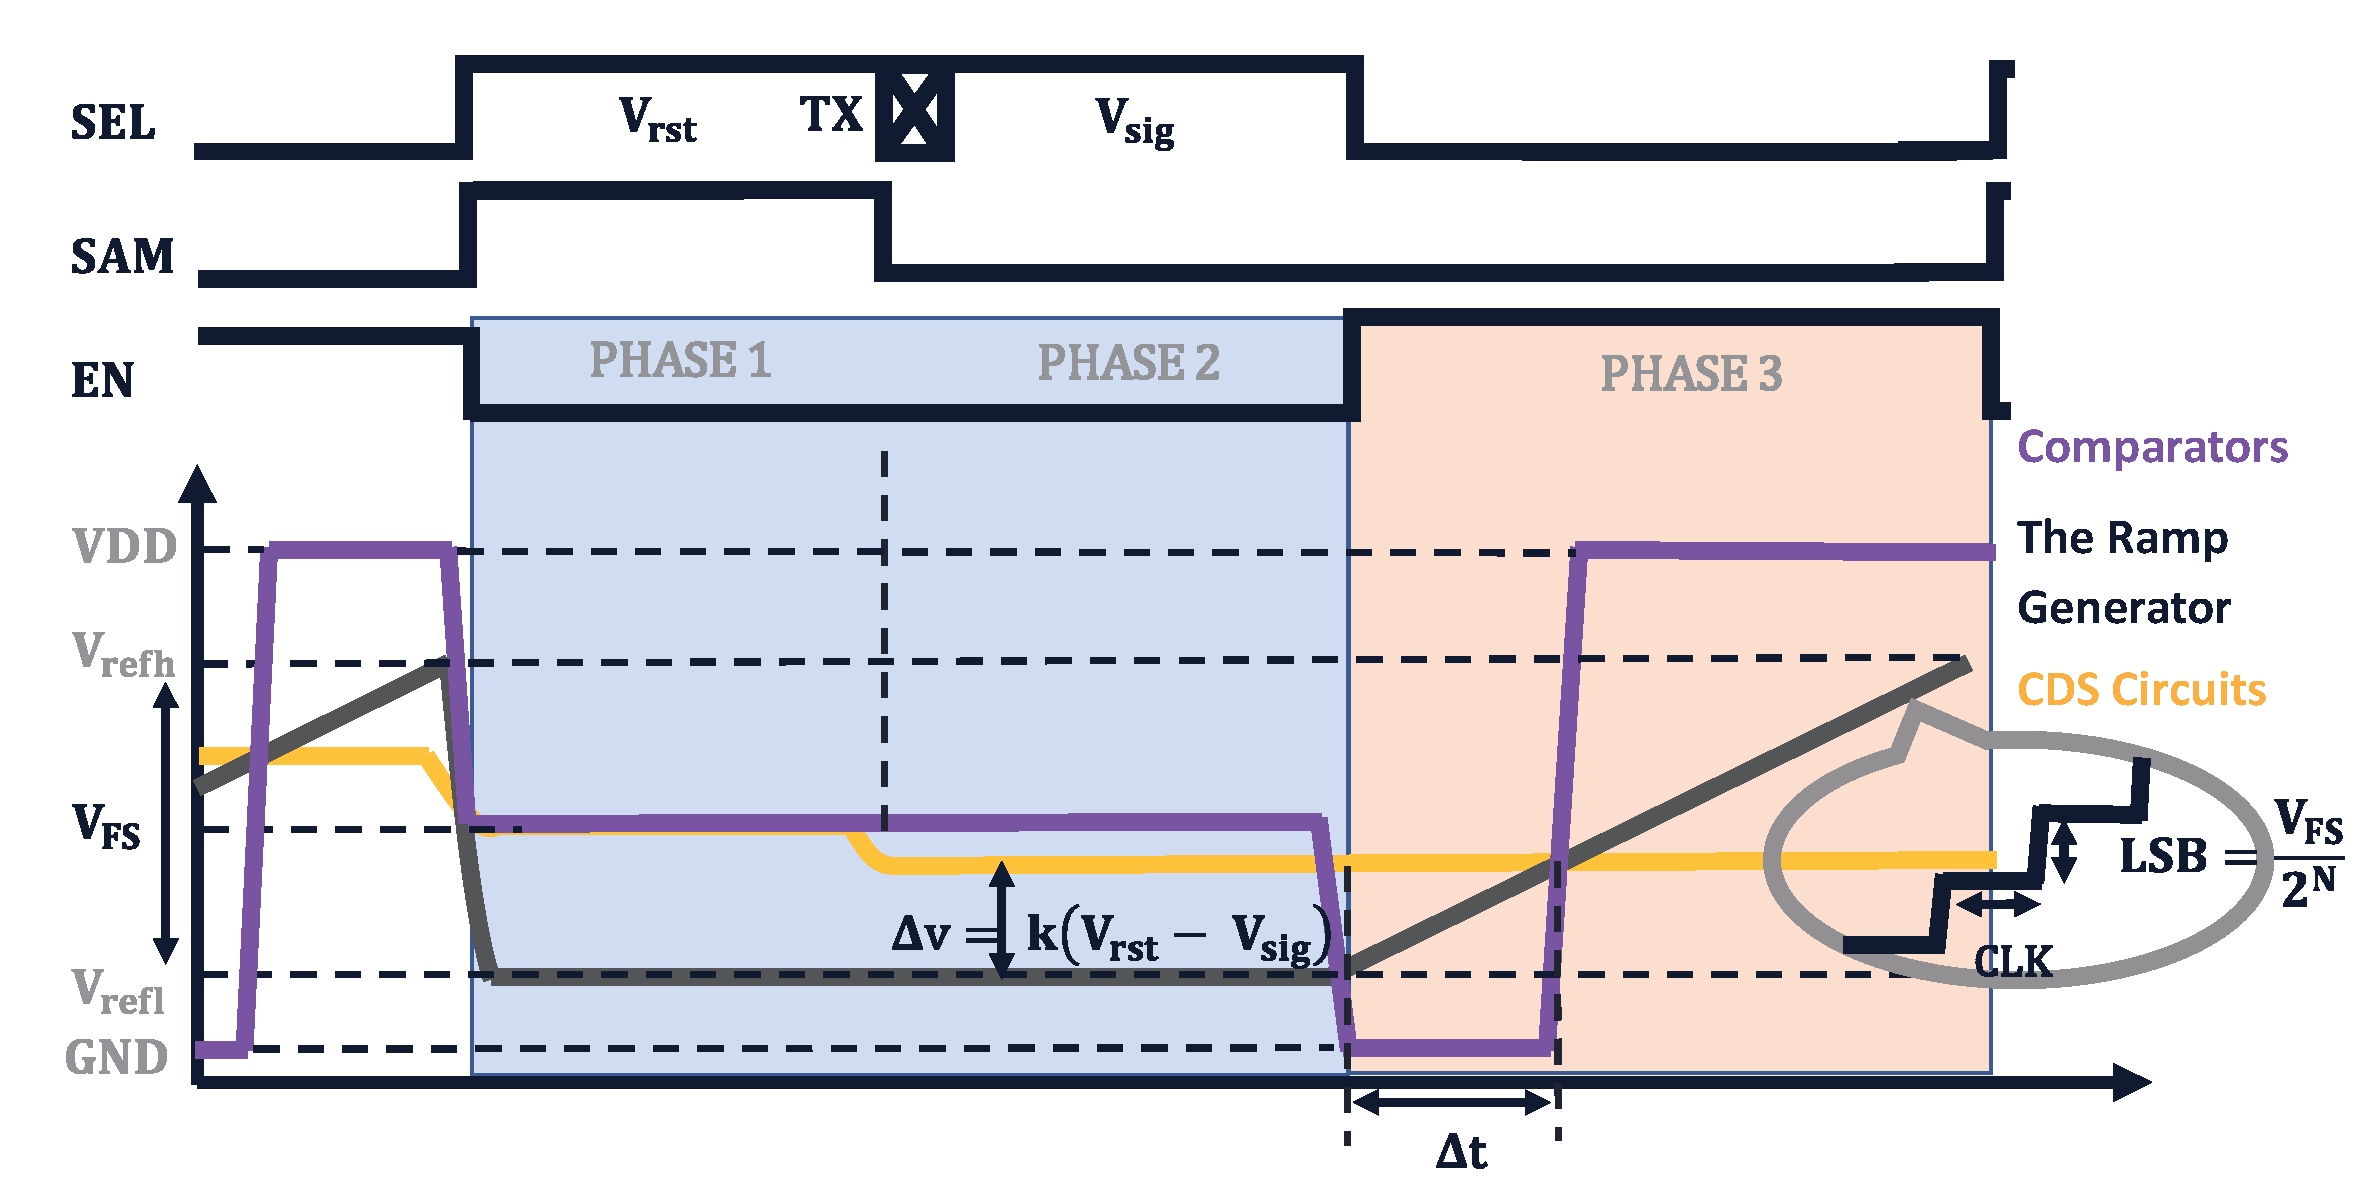
\includegraphics[width=3.5in]{./Figures/SSWAVE.eps}}
	\caption{Operational Waveform of the SS ADCs.}
	\label{SSWAVE}
\end{figure}

As the structure of the three main modules are described more specifically as follows, details of the three waves in Fig.~\ref{SSWAVE} are also revealed.

\subsubsection{CDS Circuits}

CDS circuits are the interface between the pixel array and the ADCs, responsible for subtracting the pixels’ signal voltages from reference voltages and 
amplifying the difference by a certain coefficient. The difference (i.e. $\Delta{V}$ in Fig.~\ref{SSWAVE}) is physically attached to the exposure time of the pixels, 
and the subtraction will help cancel the noises caused by the varying reference voltages. 

Switched-capacitor operational amplifiers are commonly used in CDS circuits as presented in Fig.~\ref{CDS}. According to the law of charge conservation, 
the output voltage of the CDS circuits (in PHASE2 of Fig.~\ref{SSWAVE}) can be calculated as \eqref{eq1}, consistent with the requirements. It is also noticed that the Input Offset Cancelation (IOS) is realized \cite{razavi_design_1992}, 
which is necessary because the amplifiers in different columns may have different offset voltage.

\begin{figure}[htbp]
	\centerline{\includegraphics[width=2.5in]{./Figures/CDS.eps}}
	\caption{the Structure of the CDS Circuits.}
	\label{CDS}
\end{figure} 

\begin{equation}
	\begin{aligned}
		V_{out}&=\left[ V_{ref}+\frac{C_1}{C_2}\ast\left(V_{rst}-V_{sig}\right)\right]\ast\frac{\beta A}{1+\beta A}\\
		&\;{+}\;\left(V\right._{refl}+V_{os})\ast\frac{A}{1+A}\ast\frac{1}{\beta A}\\
		&\;where\ \ \beta=\frac{C_2}{C_1+C_2}
		\label{eq1}
	\end{aligned}
\end{equation}

\subsubsection{the Ramp Generater}

As presented in Fig.~\ref{RAMP}, the ramp generator in the SS ADCs consists of a thermometer counter and a Capacitor Digital-to-Analog Converter (CDAC). 
While the capacitors in CDAC are being switched one by one from $V_{refl}$ to $V_{vefh}$, the output voltage of the ramp generator will be as \eqref{eq2} according to the law of charge conservation. 
In this equation, $N$ means the number of switched capacitors and $M$ means the total number of capacitors of the same size (for the 8-bit precision, the total number will be 255). 
Therefore, as in PHASE3 of Fig.~\ref{SSWAVE}, the ramp signal will be like stages from $V_{refl}$ to $V_{refh}$, of which the range matches with the output of CDS circuits. 
And the height of every stage is actually the Least Significant Bit (LSB) converted by the ADCs.

The three buffers in Fig.~\ref{RAMP} make sure that the reference voltages and ramp signal have enough driving capability, 
and the output buffer will be in the largest size because it has to drive hundreds of column-parallel comparators.

\begin{figure}[htbp]
	\centerline{\includegraphics[width=3.5in]{./Figures/RAMP.eps}}
	\caption{the Structure of the Ramp Generator in the SS ADCs.}
	\label{RAMP}
\end{figure} 

\begin{equation}
	V_{ramp}=V_{refl}+\frac{N}{M}\ast\left(V_{refh}-V_{refl}\right)
	\label{eq2}
\end{equation}

\subsubsection{Comparators}

The comparators work for comparing the CDS circuits' output and the ramp signal from the ramp generator. 
In the SS ADCs, two-stage open-loop comparators can be applied as presented in Fig.~\ref{COM}. Again according to the law of charge conservation, 
the comparators’ output (in PHASE3 of Fig.~\ref{SSWAVE}) can be calculated as \eqref{eq3}. The comparison will be dominated by $V_{ramp}-V_{cds}$ as long as the amplifiers’ open-loop gain 
is large enough while the IOS is also realized. In addition, the comparators’ speed relies on the amplifiers’ bandwidth and slew rate.

\begin{figure}[htbp]
	\centerline{\includegraphics[width=3.5in]{./Figures/COM.eps}}
	\caption{the Structure of the Comparators in the SS ADCs.}
	\label{COM}
\end{figure} 

\begin{equation}
	\begin{aligned}
		V_{out}&=A^2(V_{ramp}-V_{cds})\\
		&\;{+}\;\left(V_{refl}+V_{os}\right)\ast\frac{A}{1+A}\\ 		
		\label{eq3}
	\end{aligned}
\end{equation}

\subsection{Architecture of the SAR/SS ADCs}

The overall architecture of the SAR/SS ADCs is almost the same as the SS ADCs as presented in Fig.~\ref{SARADC}, and the only two differences are that the comparators are replaced by low-precision (4bit) SAR sub-ADCs and
the ramp generator is replaced by a Resistor Digital-to-Analog Converter (RDAC) with a one-hot counter.

As presented in Fig.~\ref{SAR}, a SAR sub-ADC is composed of two input buffers of the reference voltages, an array of digital-to-analog capacitors, a dynamical comparator and a module of SAR logic. While generating the upper 4-bit results, $V_{X}$ in the SAR sub-ADCs will be changed according to the SAR logic. That means after 4 comparisons 
with the reference voltage, $V_{X}$ will be as \eqref{eq4}, where $D_{U}\left[\,i\,\right]$ is the $i$ th bit of the upper 4 bits. 
And then the ramp generator will start working, making $V_{X}$ increase gradually as \eqref{eq5}, where $D_{L}\left[\,i\,\right]$ is the $i$ th bit of the lower 6 bits. 
At the time when $V_{X.2}$ exceeds $V_{ref}$, the corresponding $V_{cds}$ will be as \eqref{eq6}, which can be represented by the 10-bit conversion results, exactly.

It is worth noting that we assign 14 steps for the 4 comparisons with SAR logic. Both of the first and second comparison takes 4 steps and the following two comparison takes 3 steps. It is because that the more rapidly $V_{X}$ can be changed, the more time may required for comparison. As for the last comparison with SS logic, 1 step is enouph because $V_{X}$ will exceed $V_{ref}$ gradually, allowing the comparators to response in-time.

Fig.~\ref{RRAMP} shows the structure of the ramp generator in the SAR/SS ADCs, which consists of an R-string made up of 68 unit resistors. $V_{ramp}$ has a total number of 68 steps,
of which 64 steps with a step size of $(V_{refh}-V_{refl})/64$ are used to generate the lower 6-bit results and 4 redundant steps are used to make sure that the comparators 
will always be flipped to latch the results. In the working time, $V_{0}$ to $V_{67}$ in the ramp generator is sequentially selected as the input of the output buffer and thereby 
$V_{ramp}$ is changed from $V_{vefl}$ to $V_{vefl}+17/16(V_{refh}-V_{refl})$.

Compared to CDAC, RDAC is able to generate the ramp signal without the gain error caused by the input capacitors of the output buffer, 
which is necessary for achieving 10-bit precision in the SAR/SS mixed architecture.
Besides, the two buffers of the reference voltages in the RDAC require less energy than those in the CDAC due to less load capacitance.  

The related operational waveform of the SAR/SS ADCs is presented in Fig.~\ref{SARWAVE}. It is obvious that the upper 4-bit results (as the second last item of \eqref{eq6}) are generated 
with the SAR logic and the lower 6-bit results (as the last item of \eqref{eq6}) is counted according to the time between the ramp signal’s start and the comparators’ last flip.

\begin{figure}[htbp]
	\centerline{\includegraphics[width=3.5in]{./Figures/SARADC.eps}}
	\caption{Overall Architecture of the SAR/SS ADCs.}
	\label{SARADC}
\end{figure} 

\begin{figure}[htbp]
	\centerline{\includegraphics[width=3.5in]{./Figures/SAR.eps}}
	\caption{the Structure of the SAR Sub-ADCs in the SAR/SS ADCs.}
	\label{SAR}
\end{figure}

\begin{figure}[htbp] 
	\centerline{\includegraphics[width=3.5in]{./Figures/RRAMP.eps}}
	\caption{the Structure of the Ramp Generator in the SAR/SS ADCs.}
	\label{RRAMP}
\end{figure} 

\begin{equation}
	V_{X.1}=V_{cds}+\sum_{i=1}^{4} {\frac{V_{ref}}{2^{i}}\ast{D_{U}\left[\,i\,\right]}}
	\label{eq4}
\end{equation}

\begin{equation}
	\begin{aligned}
		&V_{X.2}=V_{X.1}+\frac{V_{ramp}}{2^4}\\ &where\  V_{ramp}=\frac{V_{ref}}{2^6-1}\ast\sum_{i=1}^{6}2^{6-i}\ast{D_{L}\left[\,i\,\right]}
		\label{eq5}
	\end{aligned}	
\end{equation}

\begin{equation}
	\begin{aligned}
		V_{cds}&=k\ast(V_{rst}-V_{sig})\\
		&\;{\approx}\;{V_{ref}-\sum_{i=1}^{4} \frac{V_{ref}}{2^{i}}\ast{D_{U}\left[\,i\,\right]}-\sum_{i=1}^{6} \frac{V_{ref}}{2^{4+i}}\ast{D_{L}\left[\,i\,\right]}}
		\label{eq6}
	\end{aligned}
\end{equation}

\begin{figure}[htbp]
	\centerline{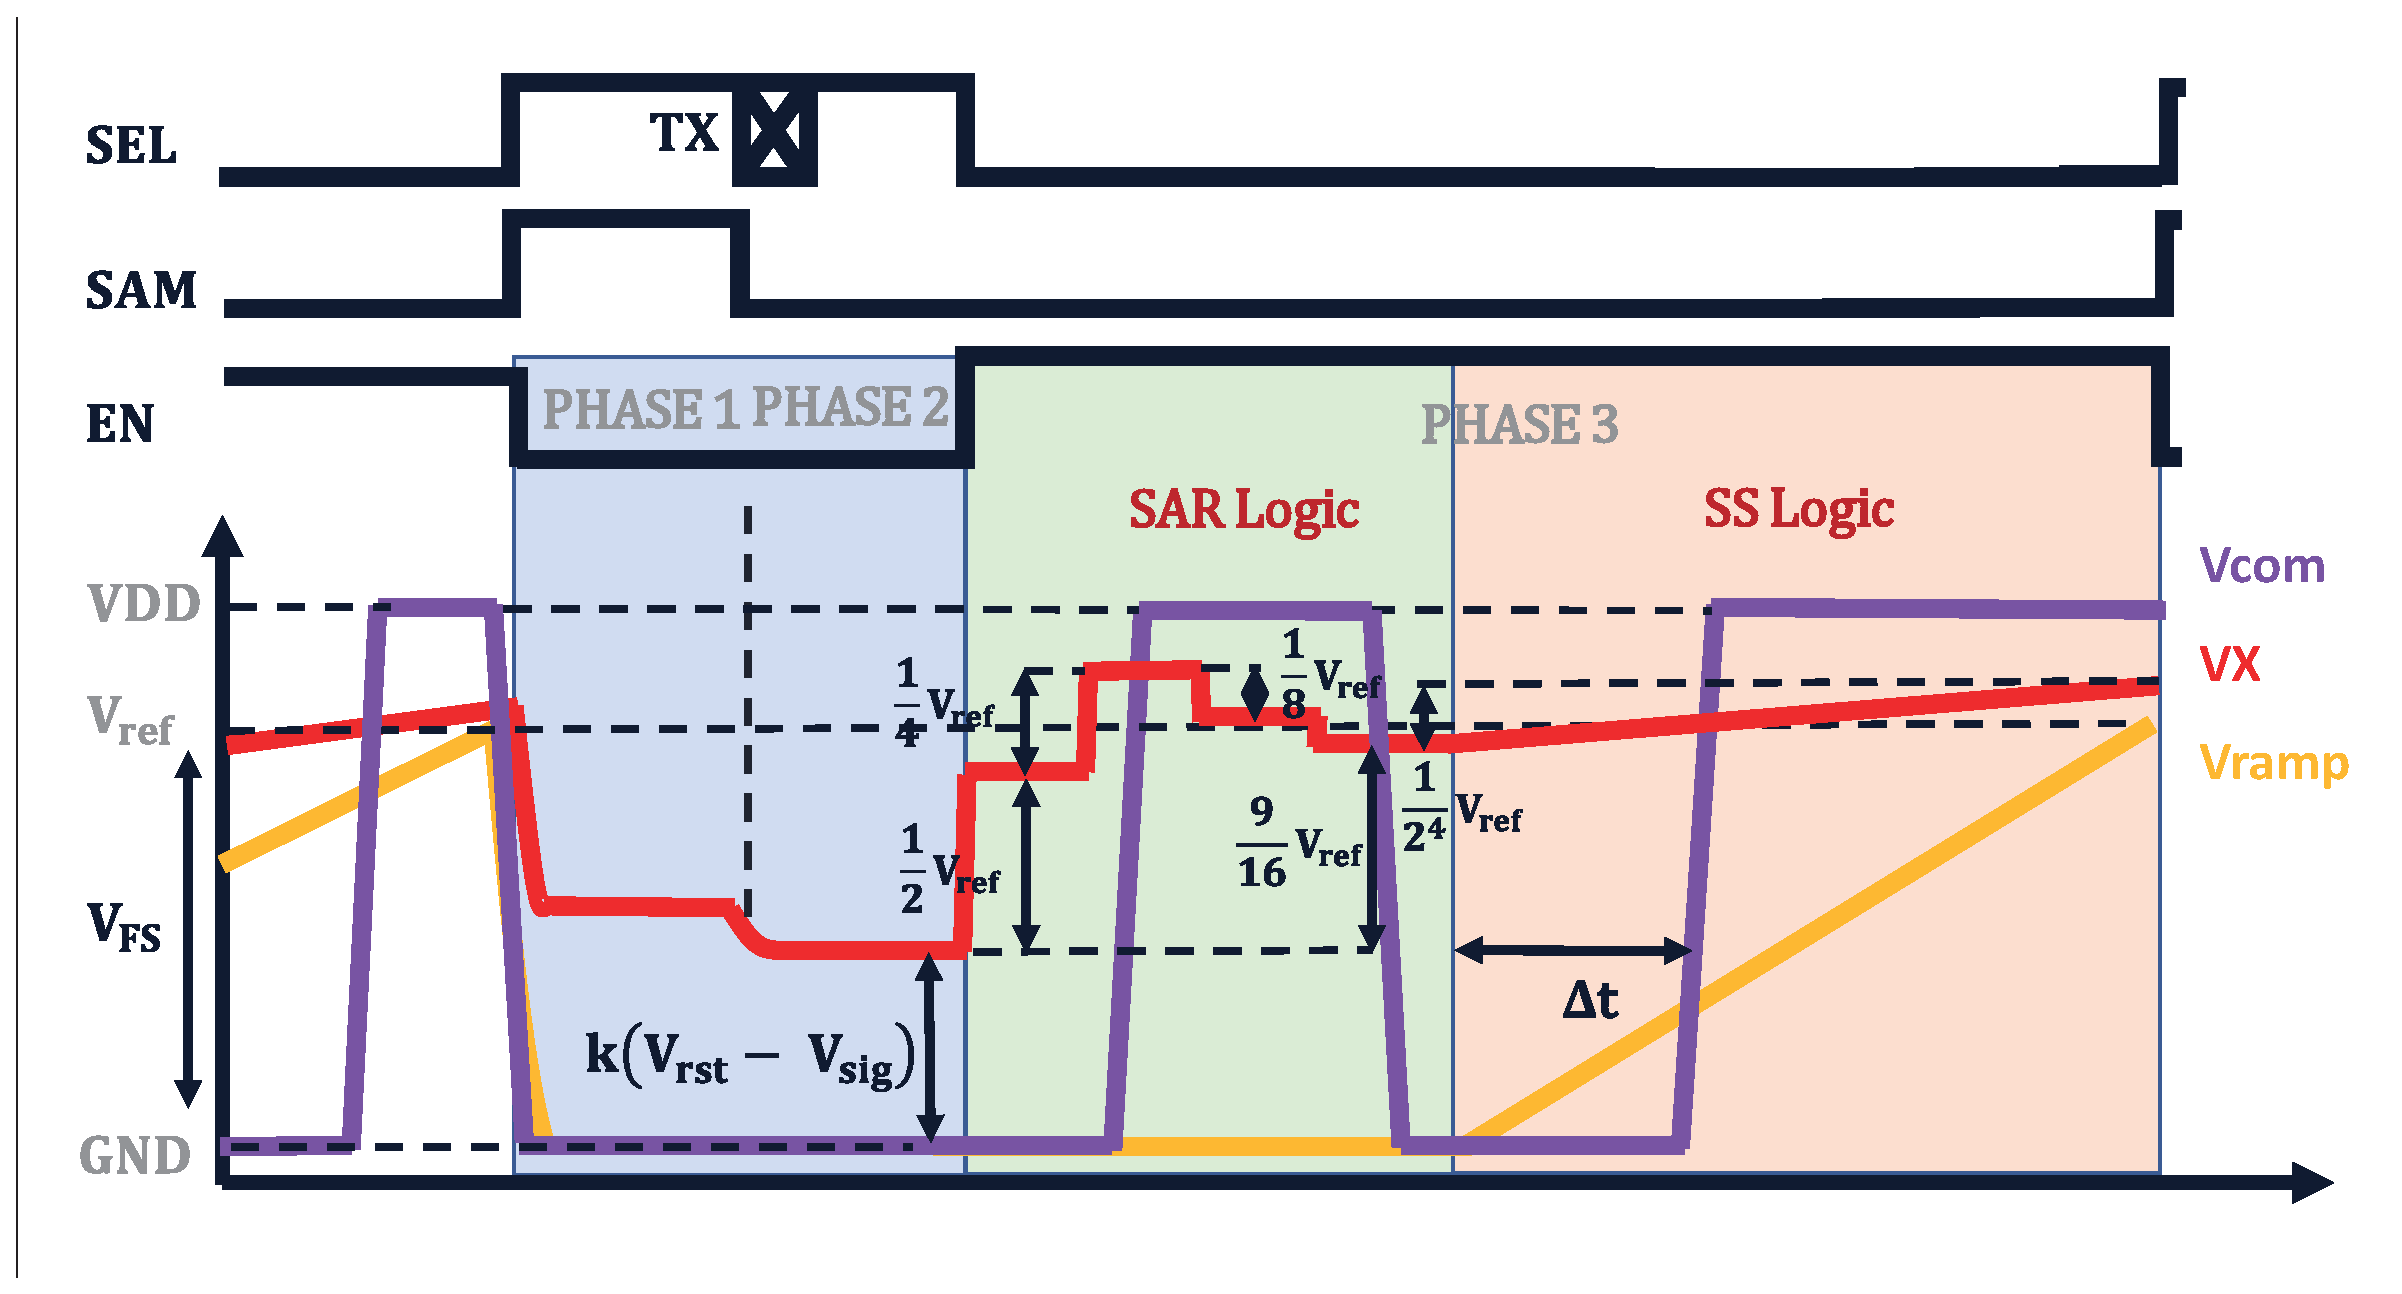
\includegraphics[width=3.5in]{./Figures/SARWAVE.eps}}
	\caption{Operational Waveform of the SAR/SS ADCs.}
	\label{SARWAVE}
\end{figure} 

As for the dynamical comparators inside the SAR sub-ADCs, traditional structure of a strong-arm comparator with pre-amplifiers is adopted as presented in Fig.~\ref{LATCH}. Such comparators 
are suitable for multiple comparisons because high speed is easy to achieve. Besides, the pre-amps’ offset voltages can be canceled effectively through the Output Offset Cancelation (OOS) \cite{razavi_design_1992}.

\begin{figure}[htbp]
	\centerline{\includegraphics[width=3.5in]{./Figures/LATCH.eps}}
	\caption{the Structure of the Comparators in the SAR Sub-ADCs.}
	\label{LATCH}
\end{figure} 

The reasons why we choose 4/8-bit adaptive-precision for the SS ADCs and 4/10-bit adaptive-precision for the SAR/SS ADCs are discussed in Sect.~\ref{discussion}.

	%\section{Implementation of Adaptive Precision and Power Gating}\label{strategy}

\subsection{Power Gating Implementation}

The power gating can be implemented simply by adding PMOS-transistor switches between the functional blocks and the supply voltage \cite{keating_low_2007} as presented in Fig.~\ref{CDS}. 
When the switches are turned off, the corresponding blocks’ current paths will be cut off and thereby the energy is saved. 

It is obvious that the more currents are under control, the more effective the power gating can be. However, to avoid unacceptable IR drop, the total size of the switches may be large, 
and inverters should be inserted between the control signal and the switches’ gates for adequate driving capability. 

Besides, the longer time the blocks can be power gated, the more energy can be saved. And a continuous long time is preferred than separated short time for power gating because
the functional blocks’ recovery speed from power off should also be taken into consideration.
As presented in Fig.~\ref{CDS}, separated short time for power gating will unavoidably waste more
time for the fuctional blocks' recovery 

Therefore, power gating will be efficient for the collumn-parallel ADCs not only due to the large sum of column-parallel currents that can be controled,
but also because that the widely adopted SS conversion logic offers exponential power scaling time.

\begin{figure}[htbp]
	\centerline{\includegraphics[width=3.5in]{./Figures/SS_pg.eps}}
	\caption{Adaptive Precision and Power Gating Implementation for the SS ADCs.}
	\label{SS_pg}
\end{figure} 

\begin{figure}[htbp]
	\centerline{\includegraphics[width=3.5in]{./Figures/SS_pg.eps}}
	\caption{Adaptive Precision and Power Gating Implementation for the SS ADCs.}
	\label{SS_pg}
\end{figure}  

\subsection{Implementation for the SS ADCs}

As evaluated in Sect.~\ref{result}, the SS ADCs’ power consumption is mainly taken up by the column-parallel comparators, bias circuits, and the output buffer of the ramp generator. 
Considering that all bias circuits are settled down only once (tens of microseconds after the whole system's power up) and then other circuits can be settled down quickly by the distributed 
bias circuits, we just apply power gating to the amplifiers in the comparators and the output buffer in the ramp generator.

The related waveform are presented in Fig.~\ref{SS_pg}. For low-precision conversion, the thermometer counter should have been extended to support switching the capacitors in CDAC 16 by 16 
rather than one by one and thereby the ramp signal will reach $V_{refh}$ in 16 steps (for 4 bits) rather than 256 steps (for 8 bits). After the 16 steps the comparators and the output buffer 
can be power gated for a long time, leaving the related signals drop gradually.

To avoid the dropping output signal of comparators causing extra unwanted latch of time information for the low-precision conversion results which should be maintained during the power off time, switches are added to the inverters fowllowing the comparators as presented in Fig.~\ref{CDS}. For power-on conversion, the two inverters' input is connected to the comparator's output, and the two inverter's output will be flipped normally as long as the comparator's output is flipped. During the power-off time, the two inverters' input is connected to the high-level power gating signal which is able to cut off the PMOS-transistor switches for energy saving. And the output signal of the two inverters will keep high-level rather than drop gradually as the comparators' output, preventing the digital latches from being unpredictable enabled and recording the time information incorrectly.

\begin{figure}[htbp]
	\centerline{\includegraphics[width=3.5in]{./Figures/SS_pg.eps}}
	\caption{Adaptive Precision and Power Gating Implementation for the SS ADCs.}
	\label{SS_pg}
\end{figure} 

\begin{figure}[htbp]
	\centerline{\includegraphics[width=3.5in]{./Figures/SS_pg.eps}}
	\caption{Adaptive Precision and Power Gating Implementation for the SS ADCs.}
	\label{SS_pg}
\end{figure} 

\subsection{Implementation for the SAR/SS ADCs}

As evaluated in Sect.~\ref{result}, the SAR/SS ADCs’ power consumption is mainly taken up by the column-parallel buffers of reference voltages in the SAR sub-ADCs.
It is because that these buffers need to drive relatively large and changing load capacitance, which means relatively large static and dynamical currents are required.
Therefore, gating these buffers will significantly reduce both static power consumption and dynamical power consumption in the ADCs.

The CDS circuits and comparators in the SAR/SS ADCs also consume a certain parts of energy. However, we only choose to take the comparators under control because they can conveniently share the same gating signal as the buffers'. And the gating signal of the buffers can also be consistent with the start signal of the ramp generator. Therefore, gating the buffers and comparators in the SAR/SS ADCs will hardly cost extra control logic but some common-used level-shifters and inverters.

Besides, the power distribution results in Sect.~\ref{result} shows that it is not necessary to take adaptive-precision adjustments inside the ramp generator of the SAR/SS ADCs, making the one-hot counter in the SAR/SS ADCs do not need to support two modes for adaptive-precision.
Therefore, compared with the SS ADCs,  the SAR/SS ADCs relatively require less adaptive-precision adjustments.

The waveform of related signals is presented in Fig.~\ref{SAR_pg}. It is noticed that For low-precison conversion, the ramp signal is generated as usaual but the buffers and comparators will be power off, leaving the 4-bit results converted completely by the SAR logic. 

As for the proportion between the power off time and the conversion time, 64/78 is achieved in the SAR/SS ADCs, which is a little less than the number 240/256 in the SS ADCs. More generally, assuming the low-precision conversion is targeting $a$ bits and the high-presision conversion is targeting $b$ bits, the corresponding equations formulating the proportion of gating time for the SS ADC s and SAR/SS ADCs will be as and , where the $k$ is a coefficient describing how many extra steps are needed for the comparison with SAR logic. Further assuming $k=4$, we can plot the proportion of gating time as in Fig.~\ref{CDS} with different $a$ and $b$ for the SS ADC s and SAR/SS ADCs. It shows that the SS ADCs are suitable for the cases where the $b-a$ are relatively small while the SAR/SS ADCs are able to have better power scaling capability for relatively large $b-a$. On the other hand, the the SS ADCs oringinally have trouble converting higher than 10 bits for full-precision because exponential increasing conversion steps will limit the throuput. Therefore, adopting SS ADCs for 4/8 adaptive-precision and SAR/SS ADCs for 4/10 adaptive-precision takes advantages and avoid weaknesses of the two different achitecture, respectively.

\begin{figure}[htbp]
	\centerline{\includegraphics[width=3.5in]{./Figures/SAR_pg.eps}}
	\caption{Adaptive Precision and Power Gating Implementation for the SAR/SS ADCs.}
	\label{SAR_pg}
\end{figure} 
	\section{Evaluation Results}\label{result}

This section presents quantitative evaluation results of the proposed adaptive-precision ADC 
designs, including a column-parallel Single-Slope (SS) ADC and a column-parallel successive 
approximation register (SAR)/SS ADC. Both ADC designs are implemented using TSMC 65nm processing,
and simulated in Virtuoso’s AMS Environment. Circuit power consumption is collectively estimated
based on the average transient current of different ADC modules given one complete sampling and 
conversion period. Power savings are then estimated by comparing the power consumption of the
low-precision conversion mode against that of the high-precision conversion mode. 

Specifically, the detailed power-breakdown and power-saving results of the proposed SS and SAR/SS ADC designs are presented in \ref{SS power} and \ref{SAR power}. And the key design characteristics are summarized in \ref{summary}, with a comparison between our work and previous reported configurable ADCs.

\subsection{Power-scaling Performance of the SS ADC Design}\label{SS power}
%Table~\ref{tab1} summarizes the key design characteristics of the SS ADC design. Considering a 
%$512\times512$ pixel array, the frame rate is 162fps.  The SNDR of the SS ADC is 23.83/46.64 dB, 
%which means the ENOB is 3.67/7.46 bits.  

Fig.~\ref{SSresults1} shows the detailed power-breakdown results of the SS ADC design,
which demonstrates that the power consumption of the SS ADC design is mainly contributed by 
the column-parallel comparators and the output buffer of the ramp generator, both of which 
can be effectively regulated via power gating for low-power conversion. The peripheral circuits include a bandgap and voltage divider, level-shift circuits and global buffers.

The power-saving results are also presented in Fig.~\ref{SSresults2}, where the annotated power consumption is measured and divided by column. It shows that the total power consumption of the low-precision conversion mode is 40.8uW/column, and the power consumption of the high-precision conversion mode is 76.2uW/column. 
Compared to the high-precision conversion mode, the low-precision conversion mode can reduce 
the power consumption approximately 50\%, which is contributed by the power-gating-regulated comparators and buffer.

\iffalse
\begin{table}[htbp]
	\caption{PERFORMANCE OF THE SS ADC DESIGN}
	\begin{center}
		\begin{tabular}{|c|c|}
			\hline
			\textbf{Prameter}& \textbf{Value} \\
			\hhline{|==|}
			\textbf{Process}& 65nm \\
			\hline 
			\textbf{Supply voltage}& 2.5/1.2 V \\
			\hline
			\textbf{Clock Frequency}&	25MHz \\
			\hline
			\textbf{Architecture}&	SS \\
			\hline
			\textbf{Quantization bits}&	4/8 bits\\
			\hline
			\textbf{Conversion time}&	12.04us \\
			\hline
			\textbf{Number of parallel columns}&	512 \\
			\hline
			\textbf{Throughput (samples per second)}&	42.5M \\ 
			\hline
			\textbf{Power (per column)}&	40.8/76.2 uW \\
			\hline
			\textbf{SNDR}& 23.83/46.64 dB@ 8.44 kHz\\
			\hline
			\textbf{ENOB}& 3.67/7.46 bits\\
			\hline
			\textbf{FOM$^{\mathrm{a}}$}& 38.59/5.21 pJ/step\\
			\hline
			\multicolumn{2}{l}{$^{\mathrm{a}}\textbf{FOM}=(\textbf{Power}\ast \textbf{Conversion}\ \textbf{time})/2^{\textbf{ENOB}}$ }	    
		\end{tabular}
		\label{tab1}
	\end{center}
\end{table}
\fi

\begin{figure}[htbp]
	\centerline{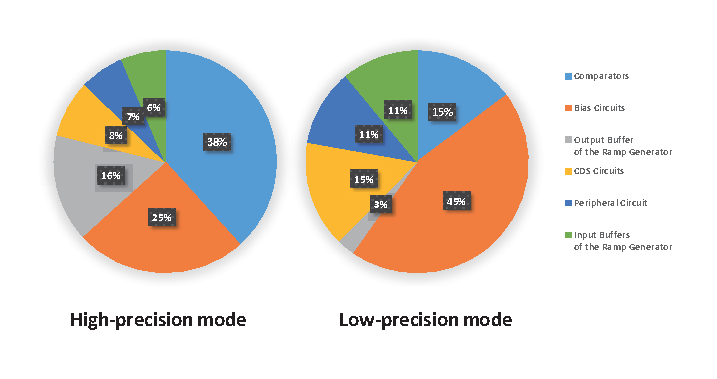
\includegraphics[width=3.5in]{./Figures/SSResults1.eps}}
	\caption{Power-breakdown results of the SS ADC design.}
	\label{SSresults1}
\end{figure}

\begin{figure}[htbp]
	\centerline{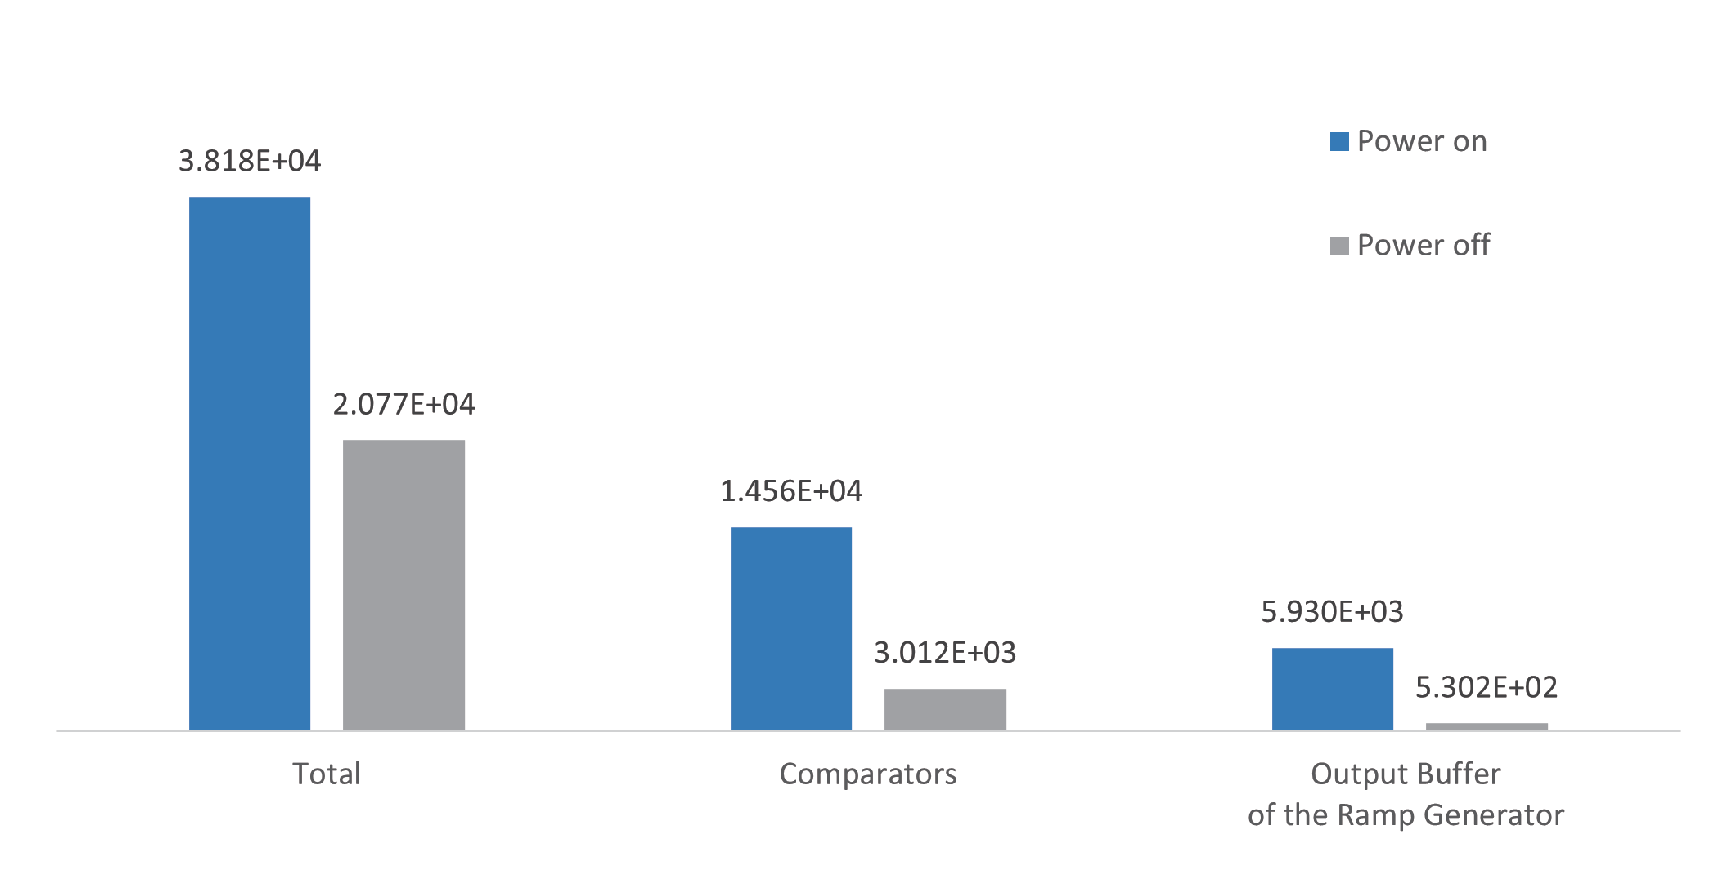
\includegraphics[width=3.5in]{./Figures/SSResults2.eps}}
	\caption{Power-saving results of the SS ADC design.}
	\label{SSresults2}
\end{figure} 

\subsection{Evaluation of the SAR/SS ADC design}\label{SAR power}

%Table~\ref{tab2} summarizes the key design characteristics of the SAR/SS ADC design, for which 
%we consider the same setup as that of the SS ADC. Since fewer steps are required in the SAR/SS ADC 
%design, 1 step is equivalent to 2 clock periods. The SNDR is 24.25/57.87 dB and the ENOB is 3.74/9.32 bits, 
%which is inline with the design specifications. 

Fig.~\ref{SARresults1} shows the detailed power-breakdown results of the SAR/SS ADC design, which 
demonstrates that the power consumption of the SAR/SS ADC design is mainly contributed by the column-parallel buffers of the reference voltages in the sub-ADCs, and power gating can effectively minimize the power consumption of these 
power-dominant components. 

The power-saving results are also presented in Fig.~\ref{SARresults2}, showing that the total power consumption of the SAR/SS ADC design is 256.1uW/column for the high-precision conversion mode and 137.1uW/column for the low-precision conversion mode. 
Compared to the high-precision conversion mode, the low-precision conversion mode can reduce the power consumption approximately 50\%.

\iffalse
\begin{table}[htbp]
	\caption{PERFORMANCE OF THE SAR/SS ADC DESIGN}
	\begin{center}
		\begin{tabular}{|c|c|}
			\hline
			\textbf{Prameter}& \textbf{Value} \\
			\hhline{|==|}
			\textbf{Process}& 65nm \\
			\hline 
			\textbf{Supply voltage}& 2.5/1.2 V \\
			\hline
			\textbf{Clock Frequency}&	20MHz \\
			\hline
			\textbf{Architecture}&	SAR/SS \\
			\hline
			\textbf{Quantization bits}&	4/10 bits \\
			\hline
			\textbf{Conversion time (us)}&	10.1us \\
			\hline
			\textbf{Number of parallel columns}&	512 \\
			\hline
			\textbf{Throughput (samples per second)}&	50.7M \\ 
			\hline
			\textbf{Power (per column)}&	137.1/256.1 uW \\
			\hline
			\textbf{SNDR}& 24.25/57.87 dB@ 10.06 kHz \\
			\hline
			\textbf{ENOB}& 3.74/9.32 bits \\
			\hline
			\textbf{FOM$^{\mathrm{a}}$}& 103.64/4.05 pJ/step\\
			\hline
			\multicolumn{2}{l}{$^{\mathrm{a}}\textbf{FOM}=(\textbf{Power}\ast \textbf{Conversion}\ \textbf{time})/2^{\textbf{ENOB}}$ }	    
		\end{tabular}
		\label{tab2}
	\end{center}
\end{table}
\fi

\begin{figure}[htbp]
	\centerline{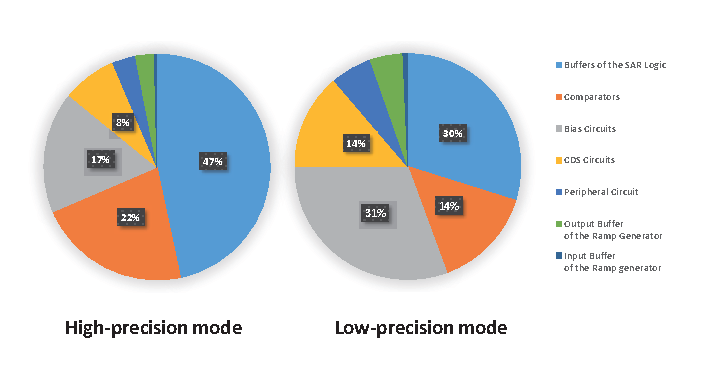
\includegraphics[width=3.5in]{./Figures/SARResults1.eps}}
	\caption{Power-breakdown results of the SAR/SS ADC design.}
	\label{SARresults1}
\end{figure} 

\begin{figure}[htbp]
	\centerline{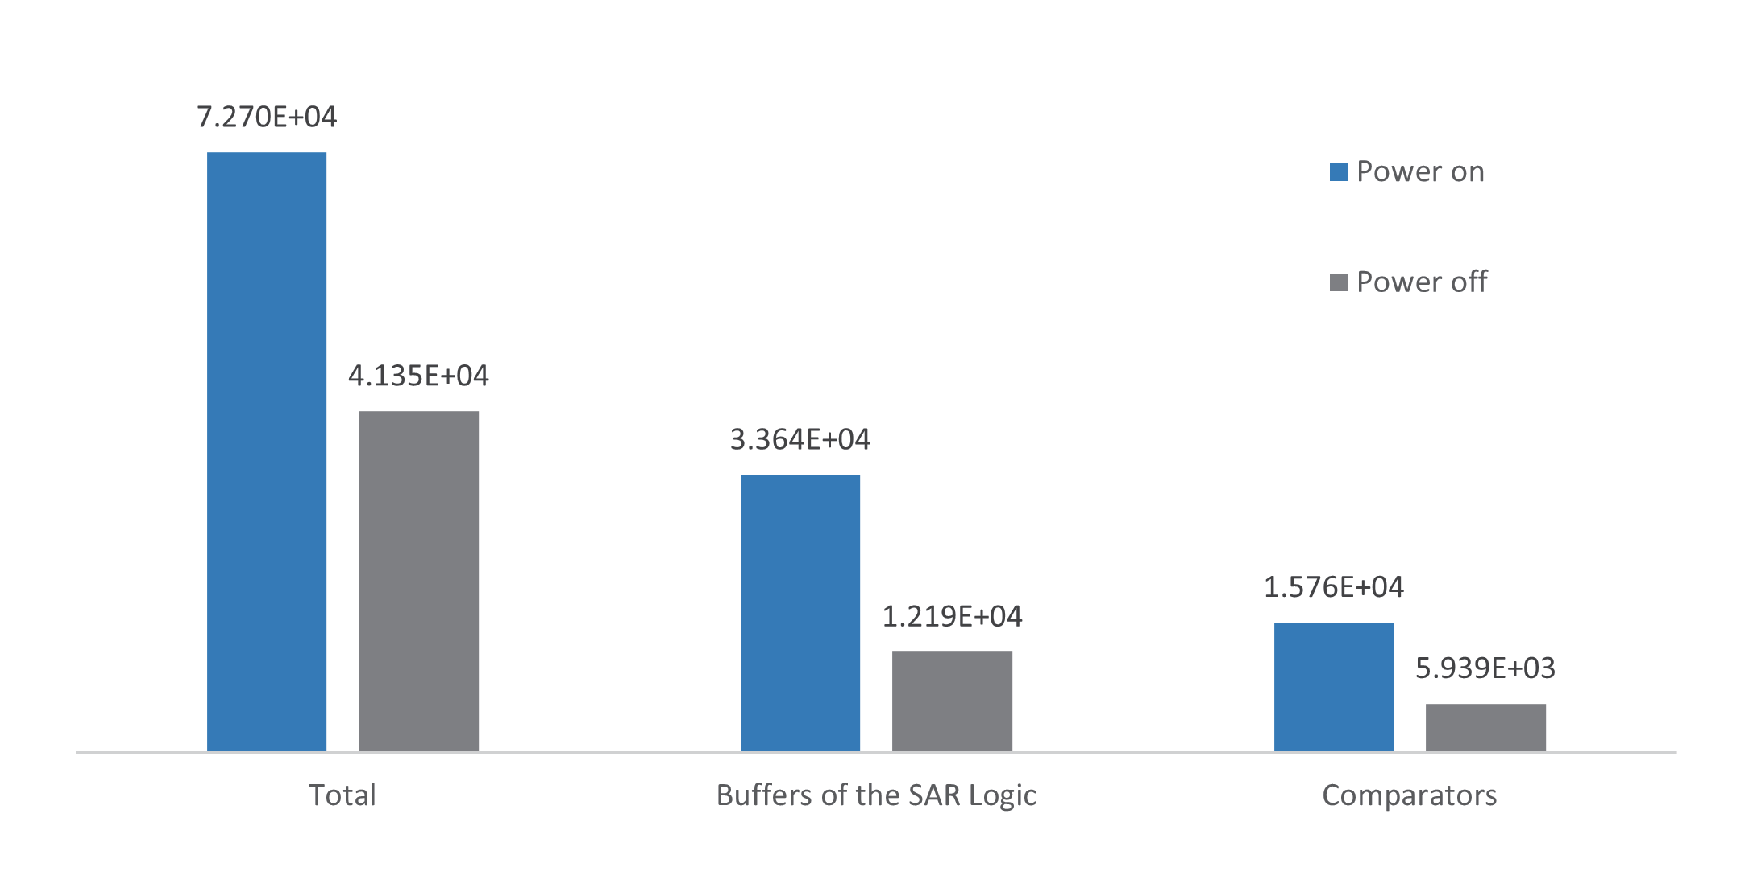
\includegraphics[width=3.5in]{./Figures/SARResults2.eps}}
	\caption{Power-saving results of the SAR/SS ADC design.}
	\label{SARresults2}
\end{figure} 

\subsection{Performance Summary and Comparison}\label{summary}

Table~\ref{tab1} summarizes the key characteristics of the proposed SS and SAR/SS ADC designs,
along with comparison of previously reported configurable ADC designs~\cite{zhu_06_2013,yip_resolution-reconfigurable_2013}. 
These prior works are chosen because they support adaptive precision and has similar precision 
and sampling rate configurations to our work. As shown in Table~\ref{tab1}, our proposed work 
achieves better power-scaling performance than the previous works. We also like to point out that
the power-scaling results reported by the prior work only consider the core ADC circuit
and ignore the peripheral circuits. Our results, on the other hand, include the complete 
design, including the bandgap, voltage divider, bias circuits and reference buffers. Therefore, 
compared to the previous work, the power-scaling performance advantage of our work should
be higher than the reported results compared to the prior works. 

It is also important to point out that the proposed power-gating method is a general one 
that can be applied to other state-of-the-art ADC architectures and realize power-efficient 
adaptive-precision ADC solutions. 

%It is highlighted that our design achieves better power-scaling performance than previous works. And the presented power-scaling percents of the SAR ADCs can actually be worse because in these works only the power consumption of the core ADC circuit is measured, while we have analysed the power consumption of the whole proposed implementation, including the bandgap, voltage divider, bias circuits and reference buffers. Therefore, with fairly considering the peripheral fixed parts of energy, the power-scaling performance of our design can definitely be more competitive.

%It is noted that the overall power consumption of the proposed implementation is relatively large with high supply voltages. However, since our design studies are targeting to exploit the power-scaling capabilities with applying reasonable power gating strategies, rather than shrinking the power consumption as more as possible for the ADCs equipped with fixed-precision, instructive power-saving effectiveness is still demonstrated.

\begin{table*}[htbp]
	\caption{PERFORMANCE SUMMARY AND COMPARISON}
	\begin{center}
		\begin{tabular}{|c|c|c|c|c|c|c|c|c|}
			\hline
			\textbf{}& \multicolumn{2}{|c|}{\cite{zhu_06_2013}} & \multicolumn{2}{|c|}{\cite{yip_resolution-reconfigurable_2013}} & \multicolumn{4}{|c|}{This work} \\
			\hhline{|=========|}
			%\iffalse
			\textbf{Process}& \multicolumn{2}{|c|}{180nm} & \multicolumn{2}{|c|}{65nm} & \multicolumn{4}{|c|}{65nm} \\
			\hline 
			\textbf{Supply voltage}& \multicolumn{2}{|c|}{0.6V} & \multicolumn{2}{|c|}{0.4V-1V} & \multicolumn{4}{|c|}{2.5V(Analog), 1.2V(Digital)} \\
			\hline
			
			%\textbf{Clock Frequency}&	20MHz \\
			%\hline
			\textbf{Architecture}& \multicolumn{2}{|c|}{SAR} & \multicolumn{2}{|c|}{SAR} & \multicolumn{2}{|c|}{SS} & \multicolumn{2}{|c|}{SAR/SS}\\
			\hline
			\textbf{Precison(bits)} & 8 & 10 & 6 & 10 & 4 & 8 & 4 & 10 \\
			\hline
			\textbf{Sampling rate(Hz)}& \multicolumn{2}{|c|}{100K} & \multicolumn{2}{|c|}{20K} & \multicolumn{2}{|c|}{83K} & \multicolumn{2}{|c|}{99K} \\
			\hline
			%\textbf{Number of parallel columns}&	512 \\
			%\hline
			%\textbf{Throughput (samples per second)}&	50.7M \\ 
			%\hline
			\textbf{SNDR(dB)} & 47.4 & 60.5 & 36.6 & 55.0 & 23.83 & 46.64 & 24.25 & 57.87 \\
			\hline
			\textbf{ENOB(bits)}& 7.58 & 9.76 & 5.79 & 8.84 & 3.67 & 7.46 & 3.74 & 9.32 \\
			\hline
			\textbf{Power consumption}& 0.32$\mu$W & 0.52$\mu$W &  0.116$\mu$W & 0.226$\mu$W & 40.8$\mu$W & 76.2$\mu$W & 137.1$\mu$W & 256.1$\mu$W\\
			\hline
			\textbf{Power-scaling performance}& 62\% & 100\% & 56\% & 100\% & \textbf{54}\% & 100\% & \textbf{54}\% & 100\% \\
			\hline
			%\fi
			%\textbf{FOM$^{\mathrm{a}}$}& 103.64/4.05 pJ/step\\
			%\hline
			%\multicolumn{2}{l}{$^{\mathrm{a}}\textbf{FOM}=(\textbf{Power}\ast \textbf{Conversion}\ \textbf{time})/2^{\textbf{ENOB}}$ }	    
		\end{tabular}
		\label{tab1}
	\end{center}
\end{table*}

	\section{Discussions}\label{discussion}
Combining adaptive-precision with fine-grained power gating strategies, both the SS ADCs and SAR/SS ADCs can save energy dynamically and significantly with only a few required control circuits. 
It is because that in the column-parallel and SS-logic-adopted ADCs, not only a large amount of currents can be under control but also the power gated time can be continously long. 

In comparison, the SAR/SS ADCs can support higher quantization bits and require fewer extra control circuits for the adaptive-precision, 
while SS ADCs inherently require less area and can be applied to the 4/8-bit situation more effectively. 
Therefore, according to specific design specifications, different structures can be chosen. 

For other different precision configurations and number of parallel collumns, 
the corresponding power consumption and energy-saving performance can also be estimated with extending the evaluation results in Sect.~\ref{result}.
	\subsection{SYSTEM-LEVEL ENERGY BENEFITS}\label{system}

Table.~\ref{tab2} further shows the energy-saving analysis for a data sensing and communicating pipeline with applying the proposed adaptive-precision ADCs. The parametric power consumption model is developed in \cite{lubana_digital_2018}, and we fit the parameters $a$, $b$ of our design into this model based on the evaluation results in \ref{result}. As we can see, the proposed adaptive-precision ADCs are able to reduce the energy of both data sensing and communication by approximately 50\%. Therefore, the proposed power gating method will be promising for improving the energy efficiency of the edge devices.

\begin{table*}[htbp]
	\caption{ENERGY-SAVING ANALYSIS FOR A SENSING AND COMMUNICATING PIPELINE WITH THE PROPOSED ADAPTIVE-PRECISION ADCS}
	\begin{center}
		\scalebox{0.7}{
			\begin{tabular}{|c|c|c|c|c|c|c|c|c|c|c|c|c|c|c|c|c|c|c|}
				\hline
				
				\multicolumn{3}{|c|}{}& \multicolumn{8}{|c|}{Image Sensor Energy} &\multicolumn{6}{|c|}{MIPI Communication Energy} &\multicolumn{2}{|c|}{Sensing\&Communication Energy} \\
				\hhline{|===================|} 			
				\hline
				\multicolumn{3}{|c|}{Formulation} & \multicolumn{8}{|c|}{$E_{sensing}=a\frac{R^2}{f}+b\frac{R}{f}+cT_{exp}$} 
				& \multicolumn{6}{|c|}{$E_{comm}={P_{comm}\left(1+h\right)\frac{pR}{BR}}$} 
				& \multicolumn{2}{|c|}{$E_{total}=E_{sensing}+E_{comm}$} \\
				
				\hline
				
				\multicolumn{3}{|c|}{Item} & \makecell[c]{$a$\\(mW/M-pixels)} & \makecell[c]{$b$\\(mW)} & \makecell[c]{$c$\\(mW)} & \makecell[c]{$R$\\(pixels)} & \makecell[c]{$f$\\(MHz)} 
				& \makecell[c]{$T_{exp}$\\($\mu$s)} & \makecell[c]{$E_{sensing}$\\(mJ)} & percent 
				& \makecell[c]{$P_{comm}$\\(mW)} & $h$ & \makecell{$p$\\(bits)} & \makecell[c]{$BR$\\(Gb/s)} & \makecell[c]{$E_{comm}$\\(mJ)} & percent
				& \makecell{$E_{total}$\\(mJ)} & percent \\ 	
				
				\hline
				
				\multicolumn{1}{|c|}{\multirow{4}*{Analysis}} & \multicolumn{1}{|c|}{\multirow{2}*{SS}} & \multicolumn{1}{|c|}{4b} & \multicolumn{1}{|c|}{70.6} & \multicolumn{1}{|c|}{2.43} & \multicolumn{1}{|c|}{\multirow{4}*{141.8}} & \multicolumn{1}{|c|}{\multirow{4}*{512$\times$512}} & \multicolumn{1}{|c|}{\multirow{2}*{42.5}} & \multicolumn{1}{|c|}{\multirow{2}*{1.8}} & \multicolumn{1}{|c|}{0.13} & \multicolumn{1}{|c|}{\multirow{2}*{\textbf{0.55}}} &
				\multicolumn{1}{|c|}{\multirow{4}*{40.7}} &
				\multicolumn{1}{|c|}{\multirow{4}*{1.35}}	& \multicolumn{1}{|c|}{4} & \multicolumn{1}{|c|}{\multirow{4}*{4}} & \multicolumn{1}{|c|}{0.0144} & \multicolumn{1}{|c|}{\multirow{2}*{\textbf{0.5}}} & \multicolumn{1}{|c|}{0.14} & \multicolumn{1}{|c|}{\multirow{2}*{\textbf{0.55}}} \\
				
				\cline{3-5} \cline{10-10} \cline{14-14} \cline{16-16} \cline{18-18}
				
				\multicolumn{1}{|c|}{} & \multicolumn{1}{|c|}{} & \multicolumn{1}{|c|}{8b} & \multicolumn{1}{|c|}{136.3} & \multicolumn{1}{|c|}{2.27} & \multicolumn{1}{|c|}{} & \multicolumn{1}{|c|}{} & \multicolumn{1}{|c|}{} & \multicolumn{1}{|c|}{} & \multicolumn{1}{|c|}{0.23} & \multicolumn{1}{|c|}{} &
				\multicolumn{1}{|c|}{} &
				\multicolumn{1}{|c|}{}	& \multicolumn{1}{|c|}{8} & \multicolumn{1}{|c|}{} & \multicolumn{1}{|c|}{0.0288} & \multicolumn{1}{|c|}{} & \multicolumn{1}{|c|}{0.26} & \multicolumn{1}{|c|}{} \\
				
				\cline{2-5} \cline{8-11} \cline{14-14} \cline{16-19}
				
				\multicolumn{1}{|c|}{} & \multicolumn{1}{|c|}{\multirow{2}*{SAR/SS}} & \multicolumn{1}{|c|}{4b} & \multicolumn{1}{|c|}{241} & \multicolumn{1}{|c|}{6.98} & \multicolumn{1}{|c|}{} & \multicolumn{1}{|c|}{} & \multicolumn{1}{|c|}{\multirow{2}*{50.7}} & \multicolumn{1}{|c|}{\multirow{2}*{1.9}} & \multicolumn{1}{|c|}{0.36} & \multicolumn{1}{|c|}{\multirow{2}*{\textbf{0.54}}} &
				\multicolumn{1}{|c|}{} &
				\multicolumn{1}{|c|}{}	& \multicolumn{1}{|c|}{4} & \multicolumn{1}{|c|}{} & \multicolumn{1}{|c|}{0.0144} & \multicolumn{1}{|c|}{\multirow{2}*{\textbf{0.4}}} & \multicolumn{1}{|c|}{0.38} & \multicolumn{1}{|c|}{\multirow{2}*{\textbf{0.53}}} \\
				
				\cline{3-5} \cline{10-10} \cline{14-14} \cline{16-16} \cline{18-18}
				
				\multicolumn{1}{|c|}{} & \multicolumn{1}{|c|}{} & \multicolumn{1}{|c|}{10b} & \multicolumn{1}{|c|}{473.5} & \multicolumn{1}{|c|}{6.98} & \multicolumn{1}{|c|}{} & \multicolumn{1}{|c|}{} & \multicolumn{1}{|c|}{} & \multicolumn{1}{|c|}{} & \multicolumn{1}{|c|}{0.68} & \multicolumn{1}{|c|}{} &
				\multicolumn{1}{|c|}{} &
				\multicolumn{1}{|c|}{}	& \multicolumn{1}{|c|}{10} & \multicolumn{1}{|c|}{} & \multicolumn{1}{|c|}{0.036} & \multicolumn{1}{|c|}{} & \multicolumn{1}{|c|}{0.71} & \multicolumn{1}{|c|}{} \\
				
				\hline
				
			\end{tabular}
		}
		\label{tab2}
	\end{center}
\end{table*}  

	\section{Conclusions}\label{conclusion}

In this work, an adaptive-precision ADC architecture to enable energy-efficient adaptive data sensing and computing for edge devices is proposed with implementation-friendly fine-grained power gating strategies.

According to the evaluation results of two CIS-applied column-parallel ADC designs, almost a half of the ADCs’ power consumption can be reduced for low-precision conversion, 
while only a few of extra control circuits is required.
It is because that in the column-parallel ADCs where the SS conversion logic is widely adopted, not only a large amount of currents can be under control but also the power gating time can be continous and exponentially scalable. 

As the proposed architecture may resonate with varying downstream deep-learning algorithms for efficient multi-tasks analysis, further works on the co-design of ADCs and algorithms remain to be developed for more intelligent edge computing in the future.
	
	\bibliographystyle{IEEEtran}
	\bibliography{main}
	
\end{document}